\begin{enumerate}
  
	\item Provide in depth detailed review of previous work on abstractions. What can be applied to 3D printing and how?
	
		I will understand \emph{abstraction} as it is defined by \cite{Mi2009}. Abstraction is an strategic simplification and elimination of detail of a shape  keeping the visual resemblance so that a viewer can still understand the shape. For example, in \cite{Berger2013} they learn a particular artist style, and use it to create abstractions of portrait photographs which resembles a sketch of that particular artist. 
		
		Particularly important for our domain is the abstraction of meshes. I will review first some works that abstract a mesh but for different purposes in fabrication. In \cite{Li2010} they take an input mesh of a building and then create an abstraction in the form of a \emph{Pop-Up} model of the building. The work of \cite{Hildebrand2012} also starts with a mesh, and they create an abstraction of it by planar cuts; it is a first step on abstraction using perceptual metric for fabrication, although their domain is very different from ours. Another example of abstraction based on meshes with the purpose of fabrication is \cite{McCrae2011}, where they create proxies from meshes with the objective of creating a puppet made of planar slices of the mesh.
		
		More related to this work is \cite{DeGoes2011}, where they create abstraction of meshes by first segmenting the mesh on meaningful patches and then lower the level of detail of each patch; their main weakness is the need of the user for the initial segmentation. A first and very basic attempt to incorporate saliency into mesh abstraction was made on \cite{Yang2009}, which is closely related to the problem. However, they only provide results from the saliency computation and not from the abstraction. 
		
		A precursor of this work is \cite{Mehra2009}; they start with an input mesh where they create a voxel hull and then they are able to make a network of curves. Their main weakness is that they claim to work only on man made objects. The work of \cite{Yumer2012}, is without a questions the closest to this one. It builds on the previous~\cite{Mehra2009}. However, instead of creating the curve network they use an implicit surfaces approach to create the abstraction which is both simpler and useful on a more general range of objects. They have also a very interesting contribution: what they call they \emph{coabstraction}; they are able to module the grade of abstraction to be able to distinguish features between a specific given set of meshes.
	
  \item Provide review of previous work on perception in CG and how it can be applied to the problem of 3D printing.
	
	In the field of digital image processing, saliency is a number assigned to each pixel in the image that represents its visual importance. In the work of \cite{Kim2010} they bridge saliency metric with the perceptions of the visual quality of a mesh. They use a centric approach based on the geometry of the mesh to make the computation and validate their results with an user study. Given a 3D scene, the work of \cite{Feixas2009} calculates the saliency of a mesh and then uses the information to find the best point of view of the scene. In the work of \cite{Wu2013}, they create a method to calculate the saliency based on local feature and a global metric that they name \emph{rarity}. They also validate their results with an user study.
	
	In the field of 3D printing, the work of~\cite{Wang2015} segments an object in pieces to optimize the printing time and at the same time use the saliency for printing the parts in an orientation to optimize the quality of the visible surface. They rely on adaptive slicing for performing this optimization which is a feature that not all the printers can made. In the other side of the spectrum to this work, is \cite{Torkhani2015}, where they claim that if the mesh changes dynamically (for example in animation) the quality can be reduced. In this sense the problem of 3D printing is the worst case, a static mesh; therefore, the visual quality is very important. Finally, the work of \cite{Echevarria2014} is an example of a work focused on 3D printing using perception metric. However, they are focused on the narrow problem of printing hair of human figurines.
	
  \item Provide detailed pipeline of your method with a detailed time line of work. What, when, and how will be completed.
	
	\begin{figure}[htp]
		\centering
    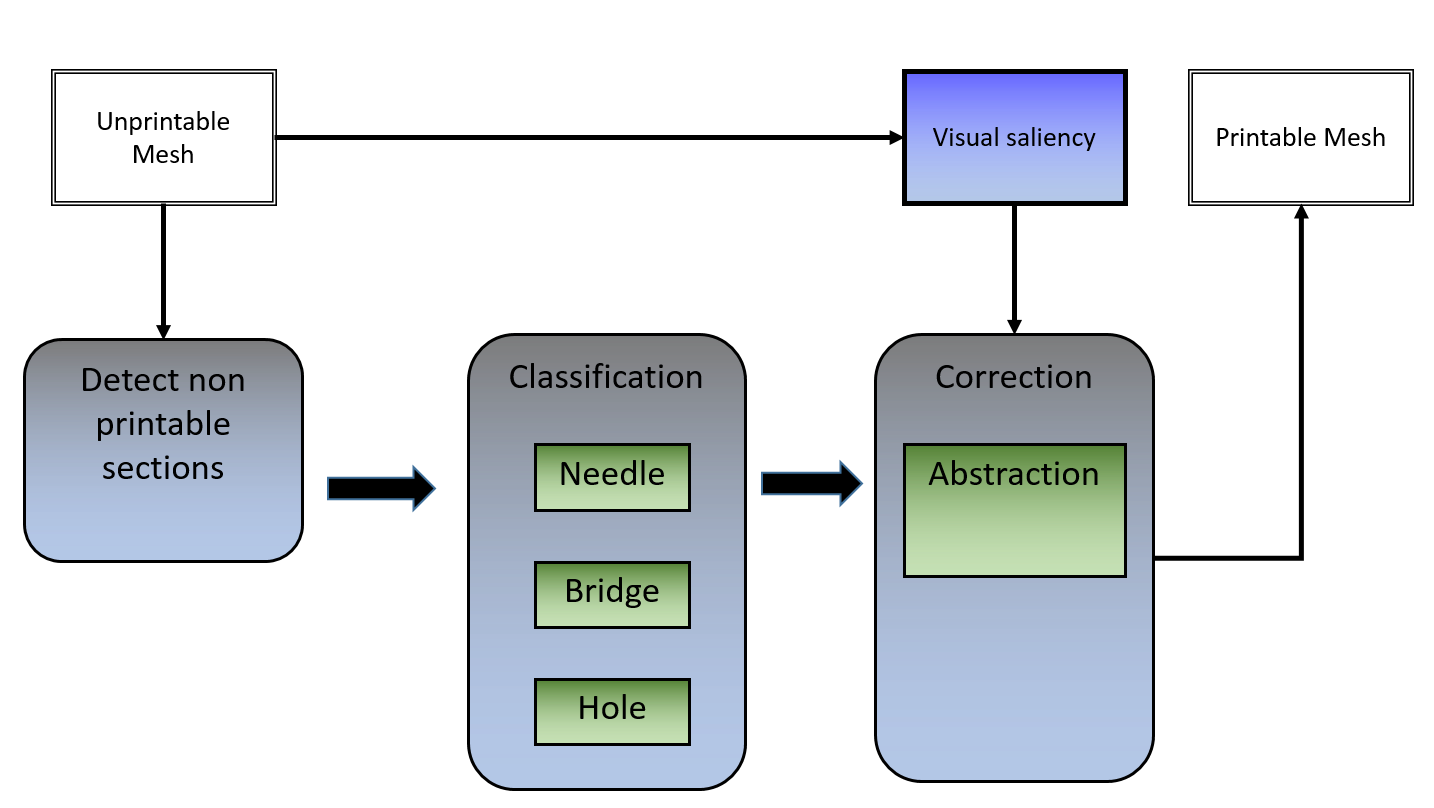
\includegraphics[width=0.85\textwidth]{img/Pipeline2}
		\caption{Proposed solution pipeline. White boxes are input and outputs. The blue box represents data and the gray boxes represent process. The green boxes represents sub process}
		\label{fig:pipeline}
	\end{figure}
	
	The overview of the solution can be seen in Figure\ref{fig:pipeline}. The input is an unprintable mesh, which is used to calculate saliency and then is processed for the automatic detection of problematic parts. As is done in~\cite{Telea2011}, we convert the input mesh in a volumetric representation and then we use morphological operations to detect features small enough to print correctly which are marked as problematic.
	
	The problematic parts are classified using their topological properties into three categories: bridges, needles and holes. Then the part is corrected by abstraction according to the corresponding category and their corresponding saliency. Finally a new mesh is extracted from the volumetric representation as a final output.
	
	\begin{center}
    \begin{tabular}{| l | r | r || p{9cm} |}
    \hline
			Task & Start date & End date & Description \\ 
			\hline
			Classify parts & May 1st & June 15th & Connected components need to be classified into three categories according his topology relative to the main mesh. See the green boxes from Figure~\ref{fig:pipeline}\\ 
			Visual saliency & August 22th & September 2nd & Visual saliency is a metric related to each vertex of the original mesh. It needs to be calculated as a guide for the abstraction process.\\ 
			Made abstraction & August 23th & October 13th & Modify the parts detected as problematic according their role and to the visual saliency. \\ 
			Re-meshing & October 13th & October 28th & The results is the original mesh plus some modified components. In this step we will need to create a way to replace parts of the original mesh with their corresponding corrected components which will broke the mesh and probably a re-meshing will be needed. \\ 
			Experiments & October 28th & September 16th & Print several examples with and without passing for my pipeline. Register the printing time and quality. \\ 
			Writing paper & October 13th & November 30th & Write the document describing the whole process. \\ 
			\hline
    \end{tabular}
	\end{center}
	
	\item What specific volumetric representation do you propose to use?
	
	I create a simple voxelization of the original mesh by inscribing the model in a simple cubic grid. In other words, we chose a $\Gamma \subset \mathbb{Z}^3$ defined as follows: 
	
		$$\Gamma = \left\lbrace \textbf{k} | A \leq k_i \leq B \text{ para } 1 \leq i \leq 3 \text{ with } A < B \text{ and } A, B \in \mathbb{Z} 	\right\rbrace $$
		
	And then, for each $\textbf{k} \in \Gamma$, we choose a positive real number $\Delta$ to define our voxels as:
	
	$$\text{Vox} (\textbf{k}) = \left\lbrace \textbf{x} \in \mathbb{R}^3 | \Delta \left(  k_i - \dfrac{1}{2} \right) \leq x_i < \Delta \left(  k_i + \dfrac{1}{2} \right)  , \text{ for } 1 \leq i \leq 3 \right\rbrace $$
	
	The set of all the voxels is our volumetric representation. The number $\Delta$ is the sampling distance. For this purpose, we set $\Delta$ to half of the printer resolution, which in our printers is $\Delta = 0.25$mm. In order to perform the voxelization we use the method described in~\cite{Nooruddin2003}, which is implemented in Binbox~\cite{Min2016}.
	
	\item What is the termination criterion? (How do you know when you are done?) Is it the user's choice, or automatic?
	
	There is no termination criteria in the sense of optimization. Rather, we detect the problematic parts, then I proceed to correct them one by one. Therefore, it finishes when there are no more problematic parts to correct. The user can choose to accept or reject the proposed abstraction, but regardless of his choice the abstraction is not recalculated.
	
	At one of the subprocess, when we produce the abstraction based on saliency there is an optimization of the metric of how far it is from the original mesh. And in that sense there is a fixed number of iterations of the abstraction as a termination criteria. Again, I would like to stress it does not make sense to become closer to the mesh than $\Delta$.

  \item Do you need to convert from volumetric representation back into to a mesh to print?
	
	Yes. In theory, this will be not necessary since most 3D printers need to slice a model and then raster each slice. Which is of course a volumetric representation. However, since we want to keep the process independent from the printer, we are not able to send the slicing directly. Instead, we convert back to a mesh representation as can be seen in Figure~\ref{fig:pipeline}. The user can send the mesh to the printer using whatever software his respective printer can use.
	
	In order to extract a mesh from the volumetric representation we use the surface tracking algorithm described in~\cite{Artzy1980}, which guaranties topology correction and fairly regular meshes.
  
	\item Can you elaborate more about this perception metric you will use to evaluate visual saliency of the 3D printed object? Are you going to verify your metric with user study? e.g. to see if user will also say that corrected model is visually plausible after the modification and there is no obvious better way how to perform the correction?
	
	This is a very interesting question. I'm not sure. The work of~\cite{Kim2010} already evaluated the quality of saliency as a perception metric in a 3D mesh; in 3D printed figurines the same result should apply. 
	
	Also, remember that the modification of the mesh is local to the problematic part. So, besides to show the difference in saliency in the original mesh and the corrected mesh; I don't know what else to measure.
	
	That being said, the user study for the final result is not completely off the table.
	
	\item How will you combine perceptual optimization with structural/material optimization? I understand we want to have optimized object that is visually plausible, but we still have to keep printability and structural strength.
	
	I’m only claiming possible contribution in the terms of printability. And I'm just measuring the printability in the terms of printer resolution. I'm aware that the result might need to be combined with a post processing step to ensure structural strength. Maybe even use the stress relive~\cite{Stava2012} as a post processing step.
	
	The structural strength extension is an interesting problem by itself. And if you don't want to modify the mesh that much abstraction sounds like a very powerful tool to attack the problem. However, right now it is out of the scope of this work.
	
	\item You mentioned that you would like to have the process interactive. I assume GPU acceleration will be used in this case. Since the model will be volumetric, how would you cope with memory restrictions put on fully volumetric (voxel) model?
	
	This is a great question too. We have two advantages:
	
\begin{itemize}
	\item First, as we can see in~\cite{Telea2011} the most expensive part should be the thin region detections. We can do it in less than 10s right now in a CPU implementation for a $1024^3$ discretization. Given the printer resolution is enough for a 20cm print.
	
	\item Second, the correction is per problematic part (a connected component), the components are handled in their morphological representation. This representation keeps track only of the object voxels, in a fashion similar to a sparse matrix. So, the memory requirements should not be as high as you mention in case we do want to make computations in the GPU.
\end{itemize}
	
	For this two reasons, I don't think that I would need to load a fully volumetric (voxel) model in GPU.
\end{enumerate}